% Paquets généraux
\documentclass[a4paper,12pt,titlepage,twoside]{article}
\usepackage[T1]{fontenc}
\usepackage[utf8]{inputenc}
\usepackage[french]{babel}
\usepackage{subcaption}
\addto\captionsfrench{%
  \renewcommand{\tablename}{Tableau}%
}
\usepackage[gen]{eurosym}
%\usepackage[dvips]{graphicx}
\usepackage{minted}
\usepackage{fancyhdr}
\usepackage{pdfpages} 
\usepackage{multido}
\usepackage{hyperref}
\usepackage{textcomp}
\usepackage{schemabloc}
%\usepackage[bitstream-charter]{mathdesign}
\usepackage{array}
\newcolumntype{P}[1]{>{\centering\arraybackslash}p{#1}}
\usepackage[shortlabels]{enumitem}
\usepackage[framemethod=TikZ]{mdframed}

\newcommand{\id}{30}
\newcommand{\nom}{Calculs d'hyperstatisme}
\newcommand{\sequence}{04}
\newcommand{\nomsequence}{Liaisons entre les solides}
\newcommand{\num}{03}
\newcommand{\type}{TD}
\newcommand{\descrip}{En appliquant les règles de la théorie des mécanisme, déterminer le degré d'hyperstatisme de plusieurs systèmes et proposer des solutions afin de diminuer ce degré}
\newcommand{\competences}{B2-12: Proposer une modélisation des liaisons avec leurs caractéristiques géométriques. \\ &  B2-13: Proposer un modèle cinématique paramétré à partir d'un système réel, d'une maquette numérique ou d'u \\ &  B2-17: Simplifier un modèle de mécanisme. \\ &  B2-18: Modifier un modèle pour le rendre isostatique.}
\newcommand{\nbcomp}{4}
\newcommand{\systemes}{E.P.A.S, Machine d'essai de traction}
\newcommand{\systemesnum}{14, 13}
\newcommand{\systemessansaccent}{E.P.A.S, Machine d'essai de traction}
\newcommand{\ilot}{3}
\newcommand{\ilotstr}{03}
\newcommand{\dossierilot}{\detokenize{Ilot_03 E.P.A.S, Machine d'essai de traction}}
\newcommand{\imageun}{EPAS}
\newcommand{\imagedeux}{Machine_dessai_de_traction}

%\usepackage{style}
\usepackage{bodegraph}
\usepackage{rpcinematik}
\usepackage[locale = FR]{siunitx}
\usepackage{caption}
\newcommand{\institute}{Lycée Dorian}
\usepackage{calc}

\usepackage{listings}
\usepackage{fancyvrb}
\usepackage{color}
\usepackage{xcolor}
\usepackage{colortbl}
\usepackage{helvet}
\usepackage[frenchmath]{newtxsf} % for sans serif symbols
\renewcommand{\familydefault}{\sfdefault}
%\usepackage{amsfonts}
%\usepackage{amsmath}
%\usepackage{lmodern}
\usepackage{mathastext}
%\usepackage{xspace}
\usepackage{varioref}
\usepackage{tabularx}
%\usepackage{floatflt}
\usepackage{graphics}
\usepackage{wrapfig}
\usepackage{textcomp}
\usepackage{tikz,tkz-tab}
\usepackage[european resistor, european voltage, european current]{circuitikz}
\usepackage{wrapfig}
\usepackage{gensymb}
\usepackage[percent]{overpic}
\usetikzlibrary{babel}
\usepackage{ifthen}
\usepackage{cancel}
\usepackage{etoolbox}
\usepackage{multirow}
%\usepackage{boxedminipage}
\definecolor{gris25}{gray}{0.75}
\definecolor{bleu}{RGB}{18,33,98}
\definecolor{bleuf}{RGB}{42,94,171}
\definecolor{bleuc}{RGB}{231,239,247}
\definecolor{bleum}{RGB}{160,195,226}
\definecolor{rougef}{RGB}{185,18,27}
\definecolor{rougec}{RGB}{255,188,204}%255,230,231
\definecolor{vertf}{RGB}{103,126,82}
\definecolor{vertc}{RGB}{220,255,191}
\definecolor{forestgreen}{rgb}{0.13,0.54,0.13}
\definecolor{blcr}{rgb}{0.59,0.69,0.84}
\definecolor{blfr}{rgb}{0.32,0.51,0.75}
\definecolor{orfr}{rgb}{0.90,0.42,0.15}
\definecolor{orcr}{rgb}{0.90,0.65,0.50}
\definecolor{orangef}{rgb}{0.659,0.269,0.072}
\definecolor{orange}{rgb}{0.58,0.35,0.063}
\definecolor{orangec}{rgb}{0.43,0.32,0.25}
\definecolor{rcorrect}{rgb}{0.6,0,0}
\definecolor{sequence}{rgb}{0.75,0.75,0.75}
\definecolor{competences}{rgb}{0.61,0.73,0.35}
\definecolor{rose}{HTML}{ff00ff}
\definecolor{grisf}{HTML}{222222}
\definecolor{grisc}{HTML}{636363}
\definecolor{normal}{HTML}{4087c4}
\definecolor{info}{HTML}{5bc0de}
\definecolor{success}{RGB}{92,184,92}
\definecolor{warning}{RGB}{240,173,78}
\definecolor{danger}{RGB}{217,83,79}
\hypersetup{                    % parametrage des hyperliens
    colorlinks=true,                % colorise les liens
    breaklinks=true,                % permet les retours à la ligne pour les liens trop longs
    urlcolor= blfr,                 % couleur des hyperliens
    linkcolor= orange,                % couleur des liens internes aux documents (index, figures, tableaux, equations,...)
    citecolor= forestgreen                % couleur des liens vers les references bibliographiques
    }

\newcolumntype{M}[1]{>{\centering\arraybackslash}m{#1}}
\definecolor{codegreen}{rgb}{0,0.6,0}
\definecolor{codegray}{rgb}{0.5,0.5,0.5}
\definecolor{codepurple}{rgb}{0.58,0,0.82}
\definecolor{backcolour}{rgb}{0.95,0.95,0.92}

\lstdefinestyle{mystyle}{
    backgroundcolor=\color{backcolour},   
    commentstyle=\color{codegreen},
    keywordstyle=\color{magenta},
    numberstyle=\tiny\color{codegray},
    stringstyle=\color{codepurple},
    basicstyle=\ttfamily\footnotesize,
    breakatwhitespace=false,         
    breaklines=true,                 
    captionpos=b,                    
    keepspaces=true,                 
    numbers=left,                    
    numbersep=5pt,                  
    showspaces=false,                
    showstringspaces=false,
    showtabs=false,                  
    tabsize=2
}

\lstset{style=mystyle}

% Mise en page
\pagestyle{fancy}

\setlength{\hoffset}{-18pt}
\setlength{\oddsidemargin}{0pt} 	% Marge gauche sur pages impaire2s
\setlength{\evensidemargin}{0pt} 	% Marge gauche sur pages paires
\setlength{\marginparwidth}{00pt} 	% Largeur de note dans la marge
\setlength{\headwidth}{481pt} 	 	% Largeur de la zone de tête (17cm)
\setlength{\textwidth}{481pt} 	 	% Largeu\textbf{r de la zone de texte (17cm)
\setlength{\voffset}{-18pt} 		% Bon pour DOS
\setlength{\marginparsep}{7pt}	 	% Séparation de la marge
\setlength{\topmargin}{-30pt} 		% Pas de marge en haut
\setlength{\headheight}{55pt} 		% Haut de page
\setlength{\headsep}{20pt} 		% Entre le haut de page et le texte
\setlength{\footskip}{30pt} 		% Bas de\textbf{ page + séparation
\setlength{\textheight}{700pt} 		% Hauteur de l'icone zone de texte (25cm)
\setlength\fboxrule{1 pt}
\renewcommand{\baselinestretch}{1}
\setcounter{tocdepth}{1}
\newcommand{\cadre}[2]
{\fbox{
  \begin{minipage}{#1\linewidth}
   \begin{center}
    #2\\
   \end{center}
  \end{minipage}
 }
}

\newcommand{\repon}[1]
{
~\ \\
\begin{tabular}{|m{\linewidth}|}
 \hline
\multido{}{#1}{\\ \hline}
\end{tabular}
}


\newcommand{\objectif}[1]{
\mdfsetup{%
frametitle={%
\tikz[baseline=(current bounding box.east),outer sep=0pt]
\node[anchor=east,rectangle,fill=bleum]
{\strut Objectif~};}}
\mdfsetup{innertopmargin=10pt,linecolor=bleum,%
linewidth=2pt,topline=true,%
frametitleaboveskip=\dimexpr-\ht\strutbox\relax
}
\begin{mdframed}[]\relax%
#1
\end{mdframed}}


\newcounter{num_quest} \setcounter{num_quest}{0}
\newcounter{num_rep} \setcounter{num_rep}{0}
\newcounter{num_cor} \setcounter{num_cor}{0}

\newcommand{\feuilleDR}[1]{
	\begin{tikzpicture}
		\draw[gray!30](0,0)grid[step=0.5cm](\linewidth,#1);
	\end{tikzpicture}
}

%\newcommand{\question}[1]{\refstepcounter{num_quest}\par
%~\ \\ \parbox[t][][t]{0.15\linewidth}{\textbf{Question \arabic{num_quest}}}\parbox[t][][t]{0.85\linewidth}{#1\label{q\the\value{num_quest}}}\par
%}

\newcommand{\question}[1]{\refstepcounter{num_quest}\par
~\ \\ \textbf{Question \arabic{num_quest} : }#1\label{q\the\value{num_quest}}\par
}

\newcommand{\posetafigure}[3]{
\begin{figure}[ht!]
 \begin{center}
  \includegraphics[width=#2\linewidth]{img/#1}
 \end{center}
 \caption{\label{#1} #3}
\end{figure}}

\newcommand{\goforum}{
\begin{figure}

\end{figure}
\begin{center}
 \includegraphics[width=0.7\linewidth]{../../../img/go_forum}
\end{center}
\label{go_forum}
\caption{J'pète les plombs}
\end{figure}}

\newcommand{\reponse}[4][1]
{\noindent
\parbox{\textwidth}{
\rule{\linewidth}{.5pt}\\
\textbf{Question\ifthenelse{#1>1}{s}{} \multido{}{#1}{%
\refstepcounter{num_rep}\ref{q\the\value{num_rep}} }:} ~\ \\
\ifdef{\public}{#3 \ifthenelse{#2>0}{~\ \\ 	\feuilleDR{#2}}}{#4}
}}

\newboolean{printdr}
\newboolean{printcor}
\setboolean{printdr}{false}
\setboolean{printcor}{false}

\newcommand{\reponseinfo}[2][1]
{\noindent
\rule{\linewidth}{.5pt}\\
\textbf{Question\ifthenelse{#1>1}{s}{} \multido{}{#1}{%
\refstepcounter{num_rep}\ref{q\the\value{num_rep}} }:} ~\ \\
\ifdef{\public}{\parbox{\textwidth}{\ifthenelse{#2>0}{~\ \\ 	\feuilleDR{#2}}}
\setboolean{printdr}{true}\setboolean{printcor}{false}}
{\setboolean{printdr}{false}\setboolean{printcor}{true}}
}

\makeatletter
\newcommand\modulo[2]{
    \newcounter{lastpagesujet}
	\setcounter{lastpagesujet}{#1}
    \divide\value{lastpagesujet} by #2
    \multiply\value{lastpagesujet} by #2
    \advance\value{lastpagesujet} by #2
    \advance\value{lastpagesujet} by 1\relax
    }
\makeatother

\newcommand{\finsujet}[1]
{
    \begin{center}
    \Large{FIN}
    \end{center}
        
    \ifthenelse{\equal{#1}{public}}{\def\public{}}{}

	\newpage

}

\newcommand{\debutcor}
{	
    \ifdef{\public}{
    	\modulo{\value{page}-1}{4}
		\whiledo{\value{page}<\value{lastpagesujet}}{~\ \newpage}
        \pagestyle{docreponse}
	}{\pagestyle{correction}}

    \ifdef{\public}{
        \begin{tikzpicture} 
            \draw (0,0) rectangle (2,2);
            \draw (0,0) -- (2,2);
            \draw (1.5,0.5) node {\large 20};
            \draw (2.5,0) rectangle (16,2);
            \draw (4.5,1.7) node {\large Commentaires:};
        \end{tikzpicture}
    }
    ~\ \\
}

%\newcommand{\repcarre}[2]
%{
%~\ \\
%\begin{tikzpicture}
%\draw [fill=white] (0,0) rectangle +(\linewidth,#1);
%\node[align=left] at (1.1,#2-0.3) {\textbf{Question #1:}};
%\end{tikzpicture}
%}

\newcommand{\titre}[1]
{\begin{center}
\cadre{0.8}{\huge #1} 
\end{center}
}


%Définition des torseurs :
\newcommand{\torseur}[2]{\left\{\mathcal{#1}_{#2} \right\}}
\newcommand{\torseurh}[3]{\left\{\genfrac{}{}{0pt}{0}{#1}{#2}\right\}_{#3}}
\newcommand{\torseurv}[8]{\left\{
\begin{matrix}
#1 & #4 \\ #2 & #5 \\ #3 &#6
\end{matrix}
\right\}_{{#7},{#8}}}

%Définition des torseurs :
%\newcommand{\torseur}[2]{\left \{\mbox{\relsize{2}{$\mathcal {#1}$}\relsize{-2}}\phantom{}_{\mbox{\scriptsize $#2$}} \right \}}
%\newcommand{\torseurh}[3]{\left\{\genfrac{}{}{0pt}{0}{#1}{#2}\right\}_{#3}}
%\newcommand{\torseurv}[8]{
%\left\{\begin{array}{@{}c|c@{}} #1 & #4 \\ #2 & #5 \\ #3 & #6 \end{array} \right\}_{#7,#8}
%}
\newcommand{\derivee}[2]{\left.\dfrac{\d #1}{\d t}\right|_{#2}}
\newcommand{\tripleint}{\int\!\!\!\!\!\int\!\!\!\!\!\int}

% Notation cinématique et statique
\newcommand{\cinematique}[2]{\mbox{#1}/\mbox{#2}}
\newcommand{\statique}[2]{\mbox{#1}\rightarrow\mbox{#2}}
\newcommand{\moment}[3]{\vv {#1}_{\scriptsize{#3}}(#2)}
\newcommand{\resultante}[2]{\vv {#1}_{\scriptsize{#2}}}


%Commande de base
\newcommand{\jo}{\left(j\omega\right)} % j \omega dans l'analyse fréquentielle
\newcommand{\tl}{\xrightarrow{\mathcal{L}}} % transformée de laplace sur fleche
\newcommand{\tli}{\xrightarrow{\mathcal{L}^{-1}}} % transformée inverse de laplace sur fleche
\renewcommand{\d}[1][]{\mathrm{d#1}}
\newcommand{\dd}[1][]{\mathrm{d#1}}
\newcommand{\vect}[2]{{#1}\wedge{#2}}
\newcommand{\base}[3]{(\vec #1,\vec #2,\vec #3)}
\newcommand{\vectbase}[4]{{\vphantom{\left| \begin{matrix}
#1\\#2\\#3 \end{matrix} \right|}}_{#4}{\left| \begin{matrix}
#1\\#2\\#3 \end{matrix} \right.}}
%Pour avoir les paragraphes sous la forme I, II, III
\renewcommand{\thesection}{\Roman{section}}
\setcounter{secnumdepth}{3}
\renewcommand{\Frlabelitemii}{$\bullet$}

% En tête et pied de page
\lhead{\nom}
\rhead{\includegraphics[width=2cm]{../../../img/logo}}
\lfoot{\auteurun,\ \auteurdeux}
\cfoot{Page \thepage}

\fancypagestyle{docreponse}{%
  \fancyhf{}
  \fancyhead[LO]{NOM Prénom: .............................}
  \rhead{\includegraphics[width=2cm]{../../../img/logo}\hspace{2pt}}
  \ifdef{\auteurdeux}{\lfoot{\auteurun,\ \auteurdeux}}{\lfoot{\auteurun}}
  \rfoot{\nom}
  \lfoot{Document réponse}
  \cfoot{Page \thepage}
   }

\fancypagestyle{correction}{%
  \fancyhf{}
  \lhead{\colorbox{danger}{\begin{minipage}{0.65\paperwidth} \textcolor{white}{\textbf{Correction}} \end{minipage}} }
  \rhead{\includegraphics[width=2cm]{../../../img/logo}}
  \lfoot{Renaud Costadoat, Françoise Puig}
  \rfoot{\colorbox{danger}{\begin{minipage}{0.3\paperwidth} \begin{flushright}\textcolor{white}{\textbf{Correction}}\end{flushright} \end{minipage}} }
  \cfoot{Page \thepage}
}

\fancypagestyle{correctioninfo}{%
  \fancyhf{}
  \lhead{\colorbox{danger}{\begin{minipage}{0.65\paperwidth} \textcolor{white}{\textbf{Correction}} \end{minipage}} }
  \rhead{\includegraphics[width=2cm]{../../../img/logo}}
  \lfoot{Renaud Costadoat, Juliette Genzmer}
  \rfoot{\colorbox{danger}{\begin{minipage}{0.6\paperwidth} \begin{flushright}\textcolor{white}{\textbf{Correction}}\end{flushright} \end{minipage}} }}

\renewcommand{\footrulewidth}{0.4pt}

\usepackage{eso-pic}
\newcommand{\BackgroundPic}{%
\put(0,0){%
\parbox[b][\paperheight]{\paperwidth}{%
\vfill
\begin{center}
\hspace{0.5cm}\vspace{0.5cm}
\includegraphics[width=\paperwidth,height=\paperheight,%
keepaspectratio]{../../../img/fond3}%
\end{center}
\vfill
}}}

\newcommand{\BackgroundPicdeux}{%
\put(25,-30){%
\parbox[b][\paperheight]{\paperwidth}{%
\vfill
\begin{center}
\includegraphics[width=\paperwidth,height=\paperheight,%
keepaspectratio]{../../../img/fond4}%
\end{center}
\vfill
}}}

\begin{document}

\pagestyle{empty}

\AddToShipoutPicture*{\BackgroundPic}

\includegraphics[width=2cm]{../../../img/logo}

\Huge{DS \numero - \sujet}

\vspace{1cm}

\ifdef{\prive}{\begin{center}\colorbox{danger}{\Huge{Avec Correction}}\end{center}}{}

\begin{center}
\centering\huge{PTSI}
\end{center}

\vspace{2cm}


\begin{center}
\centering\Large{\jour}
\end{center}

\vspace{2cm}

\normalsize

\tableofcontents

\newpage

\AddToShipoutPicture{\BackgroundPicdeux}

\pagestyle{fancy}

\begin{center}
\Huge \sujet
\end{center}


\normalsize


\paragraph{Présentation générale} ~\ \\

Ce sujet porte sur la conception d'un drone quadrirotor bio­inspiré, développé à l'institut des sciences du mouvement. Ce drone s'inspire de l'oiseau et possède la capacité de se replier en vol afin de diminuer son envergure (figures \ref{fig01} et \ref{fig02}).

En fin de repliement, les bras supportant les moteurs et hélices s'alignent le long du corps du drone pour éviter que les hélices ne touchent les bords de l'ouverture.

Cette particularité est intéressante pour des problématiques d'évitement d'obstacles dans des milieux encombrés. Le drone est de plus pourvu d'un algorithme d'estimation de taille d'obstacle en vol grâce à une perception visuelle monoculaire. Cet algorithme permet de rendre le drone plus autonome pour éviter les collisions avec son environnement et actionner son système de changement de forme si cela est nécessaire.

Tout cet ensemble constitue la plateforme Quadmorphing.

\begin{figure}[ht!]
\begin{minipage}[t]{0.49\linewidth}
\begin{center}
 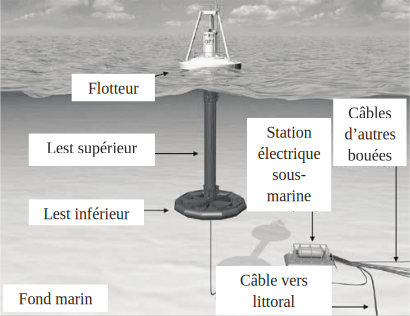
\includegraphics[width=0.95\linewidth]{img/fig01}
\end{center}
\caption{\label{fig01} L'oiseau s'adapte au passage plus étroit en modifiant son envergure}
\end{minipage}\hfill
\begin{minipage}[t]{0.49\linewidth}
\begin{center}
 \includegraphics[width=0.95\linewidth]{img/fig02}
\end{center}
\caption{\label{fig02} Vue CAO de la plateforme QuadMorphing passant à travers une ouverture}
\end{minipage}
\end{figure}

L'objectif de cette étude est de concevoir et valider les solutions technologiques retenues pour la plateforme QuadMorphing permettant le passage d'ouverture en vol. Le diagramme partiel des exigences liées à cette étude est donné en figure \ref{fig21} de l'annexe 1.

La démarche proposée est définie ci-après:
\begin{itemize}
 \item Partie I :­ Influence des mouvements des bras du drone sur son comportement.
 \item Partie II :­ Choix d'un mécanisme de modification de l'envergure.
­ \item Partie III :­ Analyse simplifiée de l'asservissement en roulis du drone.
\end{itemize}

\newpage

\section{Influence des mouvements des bras du drone sur son
comportement}

Indépendamment de la solution retenue pour mettre en mouvement les bras supportant les moteurs et hélices, nous nous intéressons dans cette partie aux conséquences des mouvements des bras sur le comportement dynamique du drone afin de valider les choix retenus par la suite.

\vspace{-0.5cm}

\subsection{Influence de la rotation des bras sur l'envergure ­ vérification des exigences Id 1 et Id 1.1}

Pour diminuer l'envergure, on choisit de replier les bras supportant les moteurs et hélices du drone. Le repliement doit être rapide et de courte durée. En effet, pour des raisons de contrôle et de stabilité, il est impossible d'utiliser un drone avec les bras repliés en permanence. La figure \ref{fig23} de l'annexe 2 présente un modèle géométrique simplifié du drone pour lequel le
bras \textbf{1}, supportant les deux moteurs et hélices avant, peut tourner par rapport au corps \textbf{0} du drone. Le bras \textbf{2}, supportant les deux moteurs et hélices arrière, peut également tourner par rapport au corps \textbf{0}. Aussi pour cette étude d'envergure, l'analyse portera sur le bras \textbf{1} seul, le comportement du bras \textbf{2} étant identique. La figure \ref{fig23} précise le paramétrage associé à cette étude. L'angle de rotation du bras \textbf{1} par rapport au corps \textbf{0} du drone est noté $\gamma_1$ et peut atteindre n'importe quelle valeur dans l'intervalle [$0\degree, 90\degree$].

L'angle de rotation du bras \textbf{2} par rapport au corps \textbf{0} du drone est noté $\gamma_2$ et peut atteindre n'importe quelle valeur dans l'intervalle [$90\degree, 180\degree$].

\question{À partir de la figure \ref{fig23} de l'annexe 2, déterminer l'expression de la largeur $\ell$ en fonction de $\gamma_1$ et des données de la géométrie du drone.}

\question{En déduire la valeur de la réduction d'envergure $A=1-\frac{\ell_{min}}{\ell_{max}}$ et l'exprimer en \%. Conclure sur la performance liée à l'exigence de réduction d'envergure Id 1.1.}

~\

Des essais expérimentaux ont été réalisés pour analyser le passage du drone au travers d'une ouverture carrée de taille de 20 cm × 20 cm et de profondeur de 1 cm. L'ouverture est placée verticalement par rapport au sol et un de ses côtés est orienté horizontalement (parallèle au sol). Selon la figure \ref{fig02}, le repère $R_G$ est associé à cette ouverture (origine $O_G$ centrée par rapport à l'ouverture).

Pour la suite, la position $\overrightarrow{O_GO}=x_G\cdot \vec{x_G}+y_G\cdot \vec{y_G}+z_G\cdot \vec{z_G}$ correspond à la position du centre d'inertie O du drone par rapport au repère $R_G$.

On définit selon les figures \ref{fig03} et \ref{fig04}, la longueur projetée $\ell_{proj}$ et la hauteur projetée $h_{proj}$ du drone dans le plan de l'ouverture. Les bords avant gauche et arrière droit du drone sont représentés respectivement par les points $\ell_{gauche}$ et $\ell_{droit}$. Les bords avant haut et arrière bas
du drone sont représentés respectivement par les points $h_{haut}$ et $h_{bas}$.

Ces grandeurs dépendent des dimensions du drone et de son orientation par rapport à $R_G$. En première approximation et en considérant un angle de roulis $\theta_R$ (rotation autour de ($O, \vec{x_0}$)) nul lors du passage de l'obstacle, la longueur projetée $\ell_{proj}$ dépend uniquement des dimensions
du drone et de l'angle de lacet $\theta_L$ (rotation autour de ($O,\vec{z_0}$)), et la hauteur projetée $h_{proj}$ dépend uniquement des dimensions du drone et de l'angle de tangage $\theta_T$ (rotation autour de ($O,\vec{y_0}$)).

\newpage

\begin{figure}[ht!]
\begin{minipage}[t]{0.49\linewidth}
\begin{center}
 \includegraphics[width=0.95\linewidth]{img/fig03}
\end{center}
\caption{\label{fig03} Définition de la longueur projetée
$\ell_{proj}$ et de l'angle de lacet $\theta_L$}
\end{minipage}\hfill
\begin{minipage}[t]{0.49\linewidth}
\begin{center}
 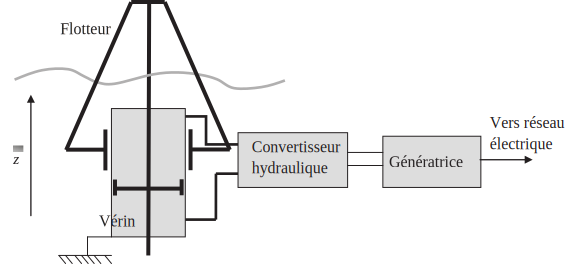
\includegraphics[width=0.95\linewidth]{img/fig04}
\end{center}
\caption{\label{fig04} Définition de la hauteur projetée
$h_{proj}$ et de l'angle de tangage $\theta_T$}
\end{minipage}
\end{figure}

Les relevés expérimentaux de 8 essais avec man\oe uvre de repliement des bras et passage de l'ouverture sont donnés en figure \ref{fig05}. La zone hachurée représente l'envergure de l'ou­verture durant toutes les positions du robot où les collisions sont possibles, c'est­-à-­dire pour $x_G \in \left[-\frac{L}{2}, \frac{L}{2}\right]$. L'aire grisée représente l'envergure maximale occupée par le drone du­rant les huit essais. Les positions des points extrêmes du drone de l'essai n°4 ($\ell_{gauche}$, $\ell_{droit}$, $h_{haut}$ et $h_{bas}$) sont représentées par les courbes avec le marqueur en forme de losange $\diamond$. On peut observer sur ces figures la diminution de l'envergure horizontale du drone à partir de la consigne de repliement (représentée verticalement en pointillés à gauche). La consigne de dépliement de la structure (représentée verticalement en pointillés à droite) est donnée dès la sortie de la zone probable de collision afin de stabiliser le drone au plus vite.

\begin{figure}[ht!]
\begin{center}
 \includegraphics[width=0.45\linewidth]{img/fig05a}
 \includegraphics[width=0.45\linewidth]{img/fig05b}
\end{center}
\caption{\label{fig05} Vues de dessus et de côté de l'envergure du drone durant huit passages de l'ouverture}
\end{figure}

\question{Relever pour l'essai n°4, la valeur de $\ell_{proj}$ avant repliement (notée $\ell_{proj}^{max}$) et la comparer à $\ell_{max}$ de la question précédente. De même pour la valeur après repliement (notée $\ell_{proj}^{min}$) à comparer à $\ell_{min}$. Si des écarts sont constatés entre les valeurs expérimentales et les valeurs théoriques, expliquer l'(les) origine(s) de ces écarts. Conclure sur la vérification de l'exigence liée au passage d'ouverture Id 1.}

\subsection{Influence de la rotation des bras sur la vitesse maximale en bout de pale ­ Vérification de l'exigence Id 4.}

On considère que le drone se déplace en ligne droite à la vitesse de déplacement $V_x\cdot \vec{x_0}$ selon $\vec{x_0}=\vec{x_G}$ telle que $V_x=2,5m\cdot s^{-1}$. Cette vitesse correspond à la vitesse retenue pour négocier
le passage de l'ouverture. Elle est suffisamment lente pour que le drone ait le temps d'interpréter la taille de l'ouverture et de décider si elle est franchissable ou non (dans ce cas le drone doit avoir le temps de réaliser un freinage d'urgence avant collision). Par ailleurs, cette vitesse est suffisamment rapide pour conserver un minimum \og d'inertie \fg lors du franchissement et permettre sa stabilisation une fois l'ouverture franchie et les bras dépliés.

Les figures \ref{fig23} et \ref{fig24} complètent le paramétrage. On suppose que le référentiel terrestre associé à $R_G$ peut être considéré galiléen. On pose de plus $\alpha=(\vec{x_1},\vec{x_{H1}})$ l'angle définissant l'orientation de l'hélice \textbf{$H_1$} par rapport au bras \textbf{1}.

La vitesse de rotation du bras \textbf{1} par rapport au corps \textbf{0} du drone, $\overrightarrow{\Omega(1/R_0)}$, est telle que $\overrightarrow{\Omega(1/R_0)}=\dot{\gamma}_1\cdot\vec{z_0}$. La valeur maximale de cette vitesse est obtenue par une rotation de $90\degree$ en
$300ms$.

La vitesse de rotation de l'hélice \textbf{$H_1$} par rapport au bras \textbf{1}, $\overrightarrow{\Omega(H1/R_1)}$, est telle que $\overrightarrow{\Omega(H1/R_1)}=\omega_1\cdot \vec{z_0}=\dot{\alpha}\cdot\vec{z_0}$. On considérera que la vitesse de rotation de l'hélice est égale à $13400tr\cdot min^{-1}$ pour assurer la portance et le déplacement horizontal du drone à $V_x=2,5m\cdot s^{-1}$.

\question{Déterminer l'expression littérale de $\overrightarrow{V(P,H1/R_G)}$, la vitesse en bout de pale de l'hélice \textbf{$H1$} par rapport à $R_G$, en fonction des données et notamment de $\dot{\gamma}_1$ et de $\omega_1$.}

\question{Dans quelle configuration du bras et de la pale cette vitesse en bout de pale est-­elle maximale ?
Déterminer dans ce cas l'expression maximale de la norme, notée $V_{max}$. Réaliser l'ap­plication numérique en déterminant au préalable la valeur numérique de chacun des termes de l'expression de $V_{max}$.
Commenter l'influence de la vitesse de rotation des bras du drone sur la valeur de $V_{max}$ et sur la vérification de l'exigence Id 4.}

\section{Choix d'un mécanisme de modification de l'envergure}

Afin de modifier la géométrie en vol, un premier mécanisme de repliement basé sur un système 4 barres a été retenu. Une modélisation de ce mécanisme est donnée en figure \ref{fig10}. La rotation du palonnier \textbf{5}, entraîné par un servomoteur d'axe ($O,\vec{z_0}$), permet la mise en rotation des bras \textbf{1} et \textbf{2} par l'intermédiaire des bielles \textbf{3} et \textbf{4}.

\begin{figure}[ht!]
\begin{center}
 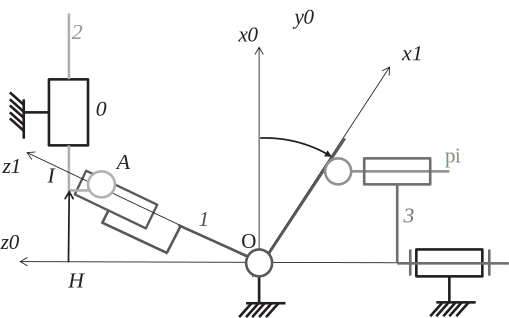
\includegraphics[width=0.75\linewidth]{img/fig10}
\end{center}
\caption{\label{fig10} Modélisation cinématique en perspective et plane en vue de dessus du mécanisme de mise en mouvement des bras du drone basé sur un double système 4 barres}
\end{figure}

\question{Réaliser le graphe de liaisons du mécanisme tel qu'il est modélisé sur le schéma cinématique de la figure \ref{fig10}.}

\question{Calculer le degré d'hyperstaticité de la modélisation spatiale du mécanisme de repliement. Détailler votre analyse en précisant selon la méthode retenue : le nombre d'équations (cinématique ou statique), le nombre d'inconnues (cinématique ou sta­tique) et le nombre de mobilités (utile et interne) en expliquant à quel(s) mouvement(s) et à quelle(s) pièce(s) ces mobilités sont associées.}

Une telle hyperstaticité impose la mise en place de jeu afin de faciliter l'assemblage. La suite va donc permettre de déterminer où placer ce jeu. On donne alors (pour le modèle de la figure \ref{fig10}, ce ne sera plus vrai dans la suite):
\begin{itemize}
 \item $\overrightarrow{OC_1}=r_5\cdot\vec{x_5}$,
 \item $\overrightarrow{A_1B_1}=-r_1\cdot\vec{x_1}$.
\end{itemize}

\question{Écrire les torseurs $\left\{V_{5/0}\right\}$, $\left\{V_{3/5}\right\}$, $\left\{V_{1/3}\right\}$ et $\left\{V_{1/0}\right\}$ en leur point d'application.}

\question{Déplacer ces torseurs au point O et écrire le système d'équations lié à la fermeture vectorielle $\left\{V_{1/3}\right\}+\left\{V_{3/5}\right\}+\left\{V_{5/0}\right\}=\left\{V_{1/0}\right\}$. En déduire les composantes hyperstatiques sur ce cycle. Cette réponse est-elle compatible avec le résultat de la question \ref{q8} ?}

\question{Proposer une modification du torseur de la liaison $\left\{V_{3/5}\right\}$ afin de rendre cette boucle isostatique. Quel serait alors le nom de la liaison ?}

~\

Pour limiter les contraintes géométriques liées au mécanisme 4 barres et afin de réduire encore le poids, le mécanisme précédent a été modifié par un mécanisme à câbles piloté par un servomoteur (figure \ref{fig11}). De plus, du fait de la dimension des bielles et des liaisons avec les bras, le mécanisme 4 barres ne permettait pas l'alignement complet des bras le long du corps (position $\gamma_1=0\degree$), ce qu'autorise désormais le mécanisme à câbles.

Ce mécanisme à câbles permet de réduire la masse du mécanisme de repliement à 6 \% de la masse totale du drone (exigence Id 1.1.2). Le servomoteur est placé au centre du drone et permet de positionner les bras à l'angle désiré. La transmission du mouvement se fait grâce aux deux câbles métalliques. Selon la figure \ref{fig25} de l'annexe 3, le câble métallique \textbf{1} est accroché d'un côté à la poulie, elle-même liée à l'axe du servomoteur, et de l'autre côté au bras \textbf{1} au point $B_1$ ; le câble métallique \textbf{2} est accroché d'un côté à la poulie et de l'autre au bras \textbf{2} au point $B_2$.

\newpage

\begin{figure}[ht!]
\begin{center}
 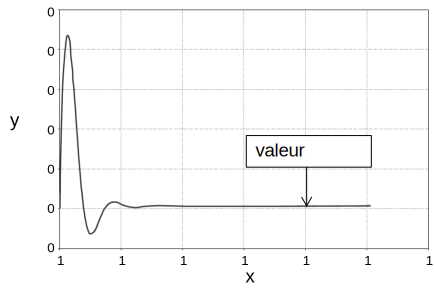
\includegraphics[width=0.65\linewidth]{img/fig11}
\end{center}
\caption{\label{fig11} Mécanisme de repliement avec servomoteur, poulie, 2 câbles métalliques et un élastique}
\end{figure}

Afin de verrouiller la structure pour n'importe quelle position des bras, un élastique relie les bras entre eux. Cet élastique est fixé aux bras du côté opposé aux points d'accroche des câbles métalliques et est guidé par l'intermédiaire d'une gorge au niveau de la poulie. La tension de l'élastique est ajustée afin de trouver un bon compromis entre le temps de repliement/dépliement des bras et la rigidité de la structure (c'est-­à-­dire l'absence de mouvement des bras durant le vol en position $\gamma_1=90\degree$).

L'étude suivante porte sur l'analyse de la loi entrée/sorties de ce mécanisme de repliement des bras présenté en figure \ref{fig25} de l'annexe 3. La loi entrée / sorties correspond à la relation entre la rotation du servomoteur et les rotations des bras du drone. L'analyse va permettre de déterminer la course angulaire à donner au servomoteur pour passer de la position bras dépliés ($\gamma_1=90\degree$) à la position bras alignés ($\gamma_1=0\degree$), mais également les dimensions géo­métriques nécessaires au bon fonctionnement du mécanisme. Le paramétrage nécessaire à cette étude est donné en annexe 3. Attention, il est différent de celui lié à la figure \ref{fig10}.

~\

Hypothèses:
\begin{itemize}
 \item ­On suppose les câbles métalliques suffisamment rigides pour pouvoir être considérés inextensibles en traction, compte tenu d'une part des efforts nécessaires pour mettre en mouvement les bras et d'autre part de l'action de l'élastique,
 \item Les câbles s'enroulent sur la poulie sans glisser,
­ \item On considère le câble non enroulé sur la poulie entre les points $C_1$ et $B_1$. Mais en réalité il l'est sur une faible portion et en toute rigueur $C_1B_1$ ne peut être considéré rectiligne.

Cette approximation permet de simplifier la géométrie du mécanisme et n'engendre
pas de grandes différences sur la valeur de la longueur du câble entre les points $C_1$ et $B_1$.
\end{itemize}

\newpage

\question{À partir du paramétrage et des hypothèses retenues, écrire la fermeture vectorielle liée à la chaîne de solides \{corps \textbf{0}, bras \textbf{1}, câble \textbf{1} et poulie \textbf{5}\}. La mettre sous la forme $L_{c1}(\theta)\cdot \vec{x_{c1}}=...$}


\question{En déduire une relation du type : $L_{c1}^2(\theta)=A\cdot cos(\gamma_A)+B\cdot sin(\gamma_1)+C$.

Exprimer les constantes $A$, $B$ et $C$ en fonction des données géométriques.}

~\

Si besoin, on donne pour la suite : $A=-11200mm^2$, $B=2400mm^2$ et $C=22100mm^2$.

\question{Déterminer approximativement la valeur numérique de $L_{c1}^{init}$ obtenue pour $\gamma_1=90\degree$ et $\theta=0\degree$. Déterminer approximativement la valeur numérique de $L_{c1}^{final}$ obtenue pour $\gamma_1=0\degree$ et $\theta=\Delta\theta$. En déduire la valeur approchée en degrés de la course angulaire $\Delta\theta$ nécessaire pour assurer le repliement du bras \textbf{1}, lorsque $\gamma_1$ passe de $90\degree$ à $0\degree$.}

~\

Avec la géométrie retenue et les positions des points d'accroche des câbles métalliques sur les bras, il est nécessaire que le câble métallique \textbf{2} soit enroulé sur la poulie avec un rayon d'enroulement $R_2$ différent de $R_1$ pour assurer que le bras \textbf{2} tourne bien de $90\degree$ lorsque la poulie tourne de $\Delta\theta$. La fermeture vectorielle de la chaîne de solides corps \textbf{0}, bras \textbf{2}, câble \textbf{2} et poulie \textbf{5} permet d'obtenir le système de deux équations suivantes pour lesquelles $R_2$ et $L_{c2}^{init}$ restent inconnues :

\begin{center}
$\left\{
\begin{array}{l}
\left(L_{c2}^{init}\right)^2=(a_2-R_2)^2+\left(\dfrac{L_0}{2}\right)^2\\
\left(L_{c2}^{init}+R_2\cdot\Delta\theta\right)^2=(\frac{L_0}{2}+a_2)^2+R_2^2
\end{array}
\right.$
\end{center}

En reliant ces deux équations à l'aide du terme $L_{c2}^{init}$, on montre que $R_2$ vérifie une équation du type $f(R_2)=0$. La figure \ref{fig12} donne l'évolution de $f(R_2)$ pour $R_2\in \left[10mm,40 mm\right]$.

\begin{figure}[ht!]
\begin{center}
 \includegraphics[width=0.75\linewidth]{img/fig12}
\end{center}
\caption{\label{fig12} Évolution de $f(R_2)$}
\end{figure}

\question{Déterminer à l'aide de la courbe de la figure \ref{fig12} une valeur approchée de $R_2$ solution du système précédent.}

~\

La valeur numérique de $L_{c2}^{init}$ correspondante est alors $L_{c2}^{init}\approx 141mm$.

Des essais à vide (hélices et drone à l'arrêt) ont été réalisés pour l'étude des performances du système de repliement/dépliement avec les dimensions déterminées précédemment. Les résultats de ces essais sont donnés en figure \ref{fig13} pour la phase de repliement et en figure \ref{fig14} pour la phase de dépliement. Sur ces courbes, le trait fort représente la valeur moyenne des positions angulaires des différents essais.

\question{Les critères de performance de l'exigence Id 1.1.2 liés au mécanisme de repliement/dépliement sont-ils respectés ?}

\question{Expliquer l'origine physique des oscillations observées sur la position angulaire du bras \textbf{1} et dans une moindre mesure sur la position angulaire du bras \textbf{2} lors du dépliement des bras.}

\begin{figure}[ht!]
\begin{center}
 \includegraphics[width=0.75\linewidth]{img/fig13}
\end{center}
\caption{\label{fig13} Relevés des angles $\gamma_1$ et $\gamma_2$ pour la phase de repliement}
\end{figure}

\begin{figure}[ht!]
\begin{center}
 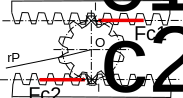
\includegraphics[width=0.75\linewidth]{img/fig14}
\end{center}
\caption{\label{fig14} Relevés des angles $\gamma_1$ et $\gamma_2$ pour la phase de dépliement}
\end{figure}

\newpage

\section{Analyse simplifiée de l'asservissement du drone}

La structure générale de commande du drone est constituée de différents éléments présentés de manière schématique en figure \ref{fig15}. On y retrouve :
\begin{itemize}
 \item le contrôleur de position qui génère les valeurs de consigne en attitude (angles de roulis $\theta_R$, de tangage $\theta_T$ et de lacet $\theta_L$) et de poussée des moteurs,
 \item le contrôleur d'attitude, qui permet de contrôler l'orientation du drone dans l'espace,
 \item  l'estimateur d'attitude, qui est composé de gyroscopes et accéléromètres pour estimer les angles de roulis $\theta_R$, tangage $\theta_T$ et d'un magnétomètre afin d'obtenir le cap du drone (angle de lacet $\theta_L$),
 \item l'estimateur de position qui est composé de la caméra embarquée et d'un baromètre afin d'estimer les positions et vitesses du drone.
\end{itemize}

L'objectif de cette partie est de vérifier que les performances de contrôle en roulis sont conservées lors du passage de l'ouverture et lors de l'activation du mécanisme de repliement/dépliement des bras. On se limite pour cela à la structure encadrée en pointillés de la figure \ref{fig15}.

\begin{figure}[ht!]
\begin{center}
 \includegraphics[width=0.85\linewidth]{img/fig15}
\end{center}
\caption{\label{fig15} Structure de commande du drone}
\end{figure}

\subsection{Modélisation du comportement des moteurs brushless}

Chaque hélice du drone est actionnée par un moteur brushless, lui-même alimenté par un ESC (Electronic Speed Controller). L'ESC est un contrôleur qui permet de faire varier la vitesse de rotation du moteur à l'aide d'une commande PPM (Pulse Position Modulation). Il génère ainsi les signaux pour les trois phases du moteur.

En vue d'établir un modèle de comportement des moteurs brushless, la vitesse de rotation du moteur $\omega_M(t)$ en $tr\cdot min^{-1}$ est mesurée pour une variation $u(t)$ de type échelon de la commande PPM de 40\% ($u(t)=0.4$) puis de 80\% ($u(t)=0.8$) sans unité. Cette évolution est donnée sur la figure du DR de la question \ref{q17}. 

Suite à cet essai, on propose de modéliser le comportement du moteur brushless par celui d'un système du 1er ordre, reliant $\Omega_M(p)$ la transformée de Laplace de la vitesse de rotation à $U(p)$ la transformée de Laplace de la commande PPM. On note $H_{mot}(p)=\frac{\Omega_M(p)}{U(p)}$ la fonction
de transfert du moteur.

\question{Justifier le modèle de comportement retenu pour Hmot (p) et déterminer ses caractéristiques (valeurs numériques et unités à préciser). Faire apparaître sur la figure du DR les tracés permettant de déterminer les caractéristiques de $H_{mot}(p)$.}

\subsection{Modélisation du comportement des hélices}

Afin d'obtenir un modèle fiable pour le contrôle du drone, les composantes de poussée T et de trainée Q de l'action de l'air sur l'hélice sont identifiées pour le couple moteur/hélice grâce à un banc d'essai. Ce banc d'essai, figure \ref{fig17}, est équipé de deux capteurs d'effort $C1$ et $C2$, chacun muni de 4 jauges de déformation, et d'un capteur optique pour mesurer la vitesse de l'hélice.

On rappelle, figure \ref{fig16}, qu'un capteur d'effort avec les jauges de déformation ainsi positionnées et orientées sur le corps d'épreuve du capteur permet d'accéder à la valeur de l'effort F appliqué sur le capteur.

\begin{figure}[ht!]
\begin{center}
 \includegraphics[width=0.35\linewidth]{img/fig16}
\end{center}
\caption{\label{fig16} Capteur d'effort. Deux jauges visibles au dessus, les deux autres en dessous}
\end{figure}

\begin{figure}[ht!]
\begin{center}
 \includegraphics[width=0.85\linewidth]{img/fig17}
\end{center}
\caption{\label{fig17} Vue et schéma du banc d'essai pour déterminer les composantes $T$ et $Q$ de l'action de l'air sur l'hélice en fonction de la vitesse de rotation de l'hélice}
\end{figure}

Les différentes mesures permettent de déterminer les évolutions de l'effort de poussée $T$ et du moment de traînée $Q$ en fonction de la vitesse de rotation $\omega_1$ de l'hélice. Ces évolutions sont présentées sur les figures du DR de la question \ref{q18}. Les mesures confirment une évolution quadratique de T et Q en fonction de $\omega_1$, avec :
\begin{center}
$T=c_T\cdot\omega_{21}^2$ avec $c_T=1\cdot 10^{-6} N\cdot rad^{-2}\cdot s^2$\\
$Q=c_Q\cdot\omega_{21}^2$ avec $c_Q=9,8\cdot 10^{-6} N\cdot m\cdot rad^{-2}\cdot s^2$,
\end{center}

où $c_T$ et $c_Q$, les coefficients de poussée, respectivement de trainée, sont obtenus par régression linéaire.

Afin de pouvoir modéliser le comportement de l'asservissement en roulis du drone lors du passage de l'ouverture, il est nécessaire de proposer un modèle de comportement linéarisé de chacun des composants du drone et notamment des hélices. On se place pour cela autour du point de fonctionnement correspondant à la vitesse d'approche du drone de l'ouverture, ce qui correspond à une vitesse de rotation des hélices de l'ordre de $1400rad\cdot s^{-1}$. On estime
que les variations de vitesse de rotation des hélices sont au maximum de $\pm 500rad\cdot s^{-1}$ lors des corrections d'attitude et de cap nécessaires au passage de l'ouverture.

\question{Proposer un modèle de comportement linéarisé de la variation de l'effort de poussée $\Delta_T$ et $\Delta_Q$ en fonction de la variation de vitesse de rotation $\Delta\omega_1$ autour du point de fonctionnement étudié ($\omega_1\approx 1400rad\cdot s^{-1}$) et valable dans le domaine de variation de
$\pm 500 rad\cdot s^{-1}$ considéré. Laisser apparents sur les courbes du DR les tracés permettant de justifier votre démarche.}

\section{Analyse du contrôleur d'attitude en roulis}

Dans cette sous-partie, on s'intéresse au réglage du contrôleur d'attitude en roulis dans le cas d'une commande en échelon sans perturbation. Puis, nous verrons comment se comporte le drone en roulis lors du passage de l'ouverture (ajout d'une perturbation) et enfin son comportement lors du repliement des bras. L'objectif est de s'assurer que le réglage du contrôleur d'attitude permet de conserver, dans une certaine mesure, le contrôle en roulis lors du passage de l'ouverture et lors du repliement/dépliement des bras.

\begin{figure}[ht!]
\begin{center}
 \includegraphics[width=0.85\linewidth]{img/fig18}
\end{center}
\caption{\label{fig18} Représentation simplifiée par schéma bloc de l'asservissement du drone en roulis, angle $\theta_R$ en degrés}
\end{figure}

L'asservissement du drone en roulis, angle $\theta_R$, est représenté par le schéma bloc de la figure \ref{fig18}. Les performances de cet asservissement sont décrites par l'exigence Id 2 du diagramme des exigences donné en figure \ref{fig21} annexe 1. Les grandeurs indiquées sur le schéma bloc de la figure \ref{fig18} représentent les transformées de Laplace des grandeurs obtenues pour des variations autour du point de fonctionnement $\theta_R=0\degree$. La vitesse de rotation du drone en roulis en $deg\cdot s^{-1}$ est notée $\Omega_R(p)$. Le contrôleur d'attitude est un correcteur de fonction de transfert $C(p)$ de sortie $U(p)$ en incréments (inc). Le comportement de l'estimateur d'angle en roulis (composé d'un gyromètre, d'un accéléromètre et d'un système de traitement des signaux) est modélisé par un gain pur $K_E$, tel que $K_E= 150 inc/deg$. ($20\cdot log(150)=43.5$).

Le bloc adaptateur, de gain pur $K_A=K_E$, permet d'adapter la consigne de variation d'angle de roulis $\theta_R^C(p)$ en degrés en une grandeur comparable à la mesure de l'estimateur d'angle de roulis.

La fonction de transfert $H_S(p)=\frac{\Omega_R(p)}{U(p)}$ représente le comportement linéarisé autour d'un point de fonctionnement (vol d'approche à vitesse constante) du drone dans la position bras déplié $\gamma_1=90\degree$. Ce comportement a été défini, entre autres, à partir des résultats des analyses des parties précédentes.

Une simulation a permis de tracer les diagrammes de Bode de la réponse fréquentielle de $H_S(p)$. Cette réponse est donnée sur la figure du DR de la question \ref{q21}, où l'on retrouve l'évolution du gain $G_{HS}(\omega)=20\cdot log|H_S(j\omega)|$ et de la phase $\Phi_{HS}(\omega)=arg(H_S(j\omega))$ en fonction de la pulsation $\omega$.

Compte tenu de la réponse fréquentielle de $H_S(p)$, on propose le modèle suivant pour $H_S(p)$ :
\begin{center}
$H_S(p)=\frac{K_S}{1+\frac{2\cdot z_S}{\omega_{0S}}\cdot p+\frac{1}{\omega_{0S}^2}\cdot p^2}$
\end{center}

\question{Justifier le choix retenu pour l'expression de $H_S(p)$ et déterminer graphiquement les valeurs numériques et unités des paramètres caractéristiques $K_S$, $z_S$ et $\omega_{0S}$. Faire apparaître sur la figure du DR, les constructions permettant de justifier les valeurs proposées.}

\question{Tracer, sur la figure du DR, les courbes de gain $G_{BO}(\omega)$ et de phase $\Phi_{BO}(\omega)$ de la réponse fréquentielle de la fonction de transfert en boucle ouverte $H_{BO}(p)=\frac{\theta_R^{mes}(p)}{\epsilon(p)}$
non corrigée, c'est à dire pour $C(p)=1$. Justifier vos tracés.}

~\

D'après les résultats des simulations, l'action proportionnelle (avec une valeur $K_p<0.1$) du contrôleur d'attitude permettrait le respect des performances en roulis dans le cas de vol non perturbé. La prise en compte des perturbations est complexe à modéliser sur un tel système, aussi on considère en première approximation que les perturbations en vol contribuent à une variation de vitesse de roulis $P(p)$, modélisée par la suite comme une perturbation de type échelon d'amplitude $P_0$
(figure \ref{fig19}).

\begin{figure}[ht!]
\begin{center}
 \includegraphics[width=0.85\linewidth]{img/fig19}
\end{center}
\caption{\label{fig19} Représentation par schéma bloc avec prise en compte des perturbations en vol}
\end{figure}

\question{Déterminer l'expression de $\theta_R(p)$ en fonction de $\theta_R^C(p)$ et de $P(p)$. On rappelle que $C(p)=K_P$ et $H_S(p)$ est définie par l'équation (2).}

\question{Déterminer l'expression de la contribution de la perturbation de type échelon d'amplitude $P_0$ sur la valeur de $\theta_R(t)$ en régime établi ($\theta_R(+\infty)$) dans le cas où la consigne est nulle $\theta_R^C(t)=0\degree$.}

\question{Quelle valeur donner à $K_P$ pour respecter le critère de précision vis-à-vis de la perturbation ? Conclure sur les limites de la correction proportionnelle.}

~\

Il est alors décidé en place une correction proportionnelle intégrale (correcteur PI) avec $C(p)=K_P\cdot\left(\frac{1+T_i\cdot p}{T_i\cdot p}\right)$. On fixe pour la suite $K_p=0,1$.

\question{Justifier que cette correction permet de satisfaire les critères de précision sur la consigne et sur la perturbation.}

~\

Les figures du DR de la question \ref{q23} donnent les résultats de la simulation du système avec la correction proportionnelle intégrale retenue. La première donne l'évolution de $\theta_R(t)$ pour une consigne de roulis $\theta_R^C(t)$ de type échelon d'amplitude $\theta_{R0}^C=10\degree$ et pour une perturbation $P(t)$ de
type échelon d'amplitude $P_0=10deg\cdot s^{-1}$ appliquée en $t=2s$. La seconde donne les courbes de gain et de phase du diagramme de Bode de la réponse fréquentielle de la FTBO corrigée.

~\

On donne les définitions suivantes:
\begin{itemize}
 \item Soit $\omega_{0dB}$ la pulsation du point de gain nul. Le système est stable en boucle fermée si, pour cette pulsation, la phase correspondante est strictement supérieure à $-180\degree$. On appelle \textbf{marge de phase}, noté $M_\varphi$, l'écart entre la valeur $-180\degree$ et la phase du point de pulsation $\omega_{0dB}$,
 \item Soit $\omega_{-180\degree}$ la pulsation du point de phase égale à $-180\degree$. Le système est stable en boucle fermée si, pour cette pulsation, le gain correspondant est strictement négatif. On appelle \textbf{marge de gain}, notée $M_G$, l'écart entre le gain du point de pulsation $\omega_{-180\degree}$ et la valeur $0dB$. 
\end{itemize}

\question{Vérifier les performances temporelles et déterminer les marges de gain et de phase de la FTBO avec correction. Faire apparaître les constructions sur les figures du DR. Conclure sur le réglage et le choix d'un correcteur PI.}

\newpage

\begin{center}
\Large{Annexe 1}
\end{center}

\begin{figure}[ht!]
\begin{center}
 \includegraphics[width=0.85\linewidth]{img/fig21}
\end{center}
\caption{\label{fig21} Diagramme partiel des exigences liées au passage de l’ouverture de la plateforme QuadMorphing.}
\end{figure}

\begin{figure}[ht!]
\begin{center}
 \includegraphics[width=0.85\linewidth]{img/fig22}
\end{center}
\caption{\label{fig22} Diagramme de définition des blocs de la plateforme QuadMorphing.}
\end{figure}

\newpage

\begin{center}
\Large{Annexe 2}
\end{center}

Notations:
La base $B_0$ associée au repère $R_0$ est notée ($O,\vec{x_0},\vec{y_0},\vec{z_0}$). Il en est de même pour le repère $R_1$ associé au bras 1 et pour le repère $R_{H1}$ associé à l’hélice $H1$. On note :
\begin{itemize}
 \item­ $\ell$ et $L$, respectivement la largeur et la longueur du parallélépipède rectangle englobant la totalité du drone (représenté en pointillés sur la figure \ref{fig23}), de hauteur $h=115mm$, constante quelle que soit la configuration du drone,
 \item $L_0=280mm$, la longueur du corps 0,
 \item $\overrightarrow{OA_1}=\frac{L_0}{2}\cdot \vec{x_0}+\frac{h}{4}\cdot \vec{z_0}$,
 \item $L_1=140mm$, la longueur du bras 1,
 \item $\overrightarrow{I_1A_1}=\frac{L_1}{2}\cdot \vec{x_1}-\frac{h}{4}\cdot \vec{z_0}$,
 \item $r_h=64mm$, la longueur d’une pale de l’hélice,
 \item $\overrightarrow{I_1P}=r_h\cdot\vec{x_{H1}}$ pour l’hélice $H1$.
\end{itemize}

\begin{figure}[ht!]
\begin{center}
 \includegraphics[width=0.95\linewidth]{img/fig23}
\end{center}
\caption{\label{fig23} Vue de dessus et en perspective du drone en phase de repliement et paramétrage de la géométrie.}
\end{figure}

\begin{figure}[ht!]
\begin{center}
 \includegraphics[width=0.55\linewidth]{img/fig24}
\end{center}
\caption{\label{fig24} Figures planes du paramétrage du bras $i$ par rapport au corps 0 du drone et de l’hélice $H1$ par rapport au bras 1 du drone.}
\end{figure}

\newpage

\begin{center}
\Large{Annexe 3}
\end{center}

\begin{figure}[ht!]
\begin{center}
 \includegraphics[width=0.3\linewidth]{img/fig25}
\end{center}
\caption{\label{fig25} Mécanisme de mise en mouvement du bras.}
\end{figure}

Notations:
\begin{itemize}
 \item l’orientation de la poulie 5 par rapport au corps du drone 0 est paramétrée par l’angle $\theta(t)$ tel que : $\theta(t)=(\vec{x_0},\vec{x_5})= (\vec{y_0},\vec{y_5})$,
 \item le rayon d’enroulement du câble métallique 1 sur la poulie 5 est noté $R_1$ , avec $R_1=30mm$. Ce rayon d’enroulement correspond à la distance $OC_1$, tel que $\overrightarrow{OC_1}=R_1\cdot y_0$,
 \item en première approximation et afin de simplifier la géométrie pour l’étude de la loi entrée/sortie de ce mécanisme, on considère la longueur $B_1C_1$ telle que $\overrightarrow{C_1B_1}=L_{c1}(\theta)\cdot \vec{x_{c1}}$, avec $
L_{c1}(\theta)=L_{c1}^{init}-R_1\cdot \theta$. La grandeur $L_{c1}^{init}$ correspond à la distance $B_1C_1$ pour $\gamma_1=90\degree$, on a
alors le point $P_1$ confondu avec $C_1$ et $\theta=0\degree$,
 \item la distance du point d’accroche $B_1$ du câble métallique 1 sur le bras 1 est notée $a_1$ telle que $\overrightarrow{A_1B_1}=-a_1\cdot \vec{x_1}$, avec $a_1=40mm$,
 \item la distance du point d’accroche $B_2$ du câble métallique 2 sur le bras 2 est notée $a_2$ telle que $\overrightarrow{A_2B_2}=a_2\cdot \vec{x_2}$, avec $a_2=a_1=40mm$,
 \item on rappelle que $\overrightarrow{OA_1}=\frac{L_0}{2}\cdot \vec{x_0}$, avec $L_0=280mm$.

On considère la position initiale du mécanisme, en configuration bras dépliés, telle que $\gamma_1=90\degree$ et $\gamma_2=90\degree$ et donc $\theta=0\degree$. On a alors $L_{c1}(\theta=0\degree)=L_{c1}^{init}$ et $L_{c2}(\theta=0\degree)=L_{c2}^{init}$.

La position finale du mécanisme est la position pour laquelle les bras sont alignés avec la direction prépondérante du drone, c’est-à-dire pour $\vec{x_1}= \vec{x_0}$ et $\vec{x_2}=-\vec{x_0}$. On a alors $\gamma_1=0\degree$,
$\gamma_2=180\degree$ et $\theta=\Delta\theta$, où $\Delta\theta$ est la course angulaire de la poulie avec $L_{c1}(\Delta\theta)=L_{c1}^{final}$ et $L_{c2}(\Delta\theta)=L_{c2}^{final}$.

\begin{center}
\Large{FIN}
\end{center}

\end{itemize}

\cleardoublepage

~\

\cleardoublepage
%\def\public

\ifdef{\public}{\pagestyle{docreponse}}{\pagestyle{correction}}

\reponse{2}{}{$\ell=2\cdot\left(r_h+\frac{L_1}{2}\cdot sin\gamma_1\right)=2.r_h+L_1\cdot sin\gamma_1$}

\reponse{3}{}{$\gamma_1=0\rightarrow \ell=\ell_{min}=2\cdot r_h$

$\gamma_1=90\rightarrow \ell=\ell_{max}=2\cdot r_h+L_1$

$A=1-\frac{l_{min}}{l_{max}}=\frac{L_1}{2\cdot r_h+L_1}=\frac{140}{140+2\times 68}\times 100>50\%$, l'id 1.1 est respectée.}

\reponse{3}{}{Bras déployés: $\ell_{proj}^{max}=0,12+0,15=0,27<l_{max}$.

Bras repliés $\ell_{proj}^{min}=0,06\times 2=0,12=l_{min}$.

Le drone n'est pas orthogonal à l'obstacle ni horizontal, cela peut expliquer ces différences. L'exigence Id 1 est bien respectée.}

\reponse{3}{}{$\overrightarrow{V_{(P, H1/Rg)}}=\overrightarrow{V_{(P, H1/1)}}+\overrightarrow{V_{(P, 1/0)}}+\overrightarrow{V_{(P, 0/Rg)}}$

$\overrightarrow{V_{(P, H1/Rg)}}=\overrightarrow{PI}\wedge\overrightarrow{\Omega_{(H1/1)}}+\overrightarrow{PA_1}\wedge\overrightarrow{\Omega_{(1/0)}}+V_x\cdot\vec{x}$

$\overrightarrow{V_{(P, H1/Rg)}}=-\frac{L_1}{2}\cdot\dot{\gamma}_1\cdot\vec{y_1}+r_h\cdot(\omega_1+\dot{\gamma}_1)\cdot \vec{y}_{H1}+V_x\cdot\vec{x}$}

\reponse{5}{}{La vitesse est maximale si toutes ses composantes sont alignées dans le même sens.

$\vec{y}_1=\vec{x}_0$ donc $\gamma_1=90$

$\vec{y}_{H1}=\vec{x}_0$ donc $\alpha=180$

$V_{max}=\frac{L_1}{2}\cdot\dot{\gamma}_1+r_h\cdot(\omega_1+\dot{\gamma}_1)+V_x$

$\dot{\gamma}_{1}^{max}=\frac{\frac{pi}{2}}{0,3}\approx 5 rad\cdot s^{-1}$

$\omega_{1}^{max}=\frac{13400\times 2\pi}{60}\approx 1340 rad\cdot s^{-1}$

$\dot{\gamma}_{1}^{max}<<\omega_{1}^{max}$

$V_{max}=2,5+70\times 10^{-3}\times 5+64\times 10^{-3}\times 1345$

$V_{max}=2,5+0,35+64\times 1,345=2,5+0,35+64+22\approx 89m\cdot s^{-1}<200m\cdot s^{-1}$ donc Id 4 ok.

}

\reponse{5}{}{
\begin{center}
  \resizebox{0.5\textwidth}{!}{\input{img/graphe_liaisons.pdf_tex}}
\end{center}}

\reponse{4}{}{
\begin{minipage}{0.45\linewidth}
$h=m-I_c+E$\\
$h=1-7+12=6$
\end{minipage}\hfill
\begin{minipage}{0.45\linewidth}
$h=Ns-rs=Ns-6(p-1)+m$\\
$h=35-30+1=6$
\end{minipage}}

\reponse{10}{}{
$\left\{V_{5/0}\right\}=\left\{\begin{array}{cc}
0&0\\0&0\\\omega_{50}&0
\end{array}\right\}_O$

$\left\{V_{3/5}\right\}=\left\{\begin{array}{cc}
0&0\\0&0\\\omega_{35}&0
\end{array}\right\}_{C_1}$

$\left\{V_{1/3}\right\}=\left\{\begin{array}{cc}
0&0\\0&0\\\omega_{13}&0
\end{array}\right\}_{B_1}$

$\left\{V_{1/0}\right\}=\left\{\begin{array}{cc}
0&0\\0&0\\\omega_{10}&0
\end{array}\right\}_{A_1}$
}

\ifdef{\public}{\newpage}

\reponse{10}{}{
$\left\{V_{3/5}\right\}=\left\{\begin{array}{cc}
0&r_5\cdot sin\theta_5\cdot\omega_{35}\\0&-r_5\cdot cos\theta_5\cdot\omega_{35}\\\omega_{35}&0
\end{array}\right\}_O$

$\left\{V_{1/3}\right\}=\left\{\begin{array}{cc}
0&-r_1\cdot sin\theta_1\cdot\omega_{13}\\0&(-\frac{L_0}{2}+r_1\cdot cos\theta_1)\cdot\omega_{13}\\ \omega_{13}&0
\end{array}\right\}_O$

$\left\{V_{1/0}\right\}=\left\{\begin{array}{cc}
0&0\\0&-\frac{L_0}{2}\cdot\omega_{10}\\\omega_{10}&0
\end{array}\right\}_O$

$\left\{\begin{array}{l}
0=0+0+0\\
0=0+0+0\\
\omega_{10}=\omega_{13}+\omega_{35}+\omega_{50}\\
0=-r_1\cdot sin\theta_1\cdot\omega_{13}+r_5\cdot sin\theta_5\cdot\omega_{35}+0\\
-\frac{L_0}{2}\cdot\omega_{10}=(-\frac{L_0}{2}+r_1\cdot cos\theta_1)\cdot\omega_{13}-r_5\cdot cos\theta_5\cdot\omega_{35}+0\\
0=0+0+0
\end{array}
\right.$

Les composantes hyperstatiques sont $\omega_x$, $\omega_y$ et $V_x$, on retrouve bien un hyperstatisme de 3.
}

\reponse{4}{}{On peut ajouter ces 3 composantes à la liaison de 3/5.

$\left\{V_{3/5}\right\}=\left\{\begin{array}{cc}
\omega_x&r_5\cdot sin\theta_5\cdot\omega_{35}\\\omega_x&-r_5\cdot cos\theta_5\cdot\omega_{35}\\\omega_{35}&V_x
\end{array}\right\}_O$

On reconnaît alors une linéaire annulaire.}


\reponse{5}{}{On a: $\overrightarrow{OA_1}+\overrightarrow{A_1B_1}+\overrightarrow{B_1C_1}+\overrightarrow{C_1O}=\vec{0}$

$\frac{L_0}{2}\cdot\vec{x_0}-a_1\cdot\vec{x_1}-L_{c1}(\theta)\cdot\vec{x_{c1}}-R_1\cdot\vec{y_0}=\vec{0}$

$L_{c1}(\theta)\cdot\vec{x_{c1}}=\frac{L_0}{2}\cdot\vec{x_0}-a_1\cdot\vec{x_1}-R_1\cdot\vec{y_0}$}

\reponse{7}{}{$L_{c1}(\theta)^2=\left(\frac{L_0}{2}\cdot\vec{x_0}-a_1\cdot\vec{x_1}-R_1\cdot\vec{y_0}\right)\cdot\left(\frac{L_0}{2}\cdot\vec{x_0}-a_1\cdot\vec{x_1}-R_1\cdot\vec{y_0}\right)$


$L_{c1}(\theta)^2=\left(\frac{L_0}{2}\right)^2+a_1^2+R_1^2-L_0\cdot a_1\cdot cos\gamma_1+2\cdot a_1\cdot R_1\cdot sin\gamma_1$

Donc, $A=-L_0\cdot a_1$, $B=2\cdot a_1\cdot R_1$ et $C=\left(\frac{L_0}{2}\right)^2+a_1^2+R_1^2$}

\reponse{7}{}{$L_{c1}^{init}=\sqrt{B+C}=\sqrt{2400+22100}=\sqrt{24500}\approx 10\times 5\times\sqrt{10}\approx 150mm$

$L_{c1}^{final}=\sqrt{A+C}=\sqrt{-11200+22100}=\sqrt{10900}\approx 100mm$

$L_{c1}^{final}=L_{c1}^{init}-R_1\cdot\Delta\theta$

$\Delta\theta=\frac{L_{c1}^{init}-L_{c1}^{final}}{R_1}=\frac{150-100}{30}=\frac{50}{30}\approx 1+\frac{2}{3}\approx 1,66rad\approx 95\degree$
}

\reponse{5}{}{Par lecture, $R_2=23mm$, (intersection avec le 0).}

\ifdef{\public}{\newpage}

\reponse{5}{}{
\begin{itemize}
 \item impossible de conclure sur la rigidité,
 \item rapidité : le temps de réponse est de 200ms<300ms
 \item précision : erreur de position est nulle : OK,
 \item poids : 6\% du poids total : OK
\end{itemize}}

\reponse{2}{}{Les vibrations sont sans doute expliquées par la présence des élastiques.}


\reponse{6}{\begin{center}
	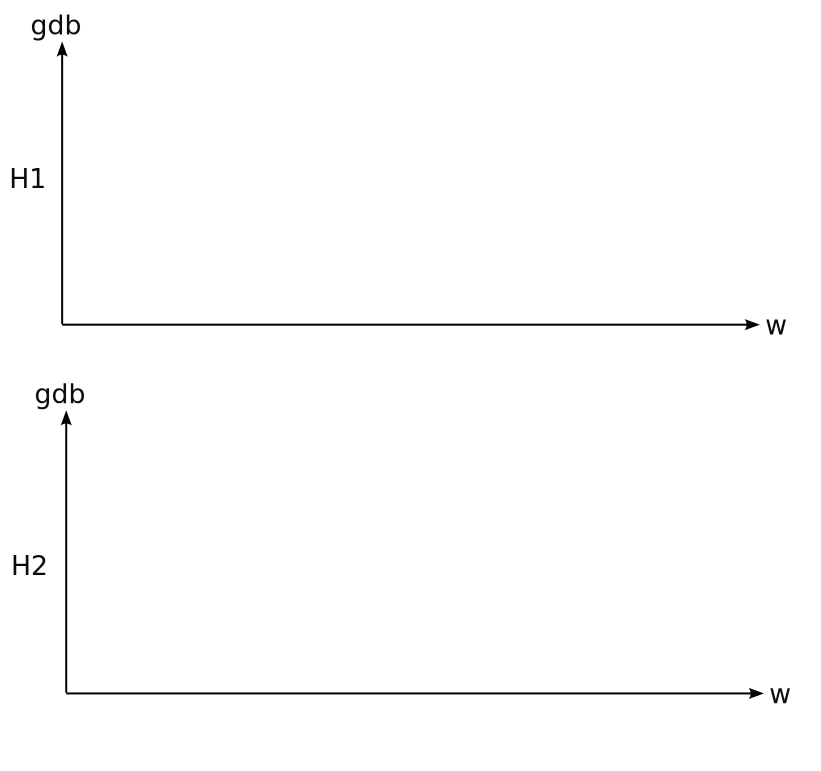
\includegraphics[width=0.6\linewidth]{img/dr01}
\end{center}}{\begin{center}
  \resizebox{0.8\textwidth}{!}{\input{img/dr01_cor.pdf_tex}}
\end{center}
Par lecture:
\begin{itemize}
 \item 1er ordre,
 \item $\tau_{mot}\approx 0,06s$,
 \item $10000=0.4\cdot K_{mot}\rightarrow K_{mot}=25000tr\cdot min^{-1}\approx 2500rad\cdot s^{-1}$.
\end{itemize}

La fonction de transfert est donc : $\frac{\Omega_M(p)}{U(p)}=\frac{2500}{1+0,6\cdot p}$.
}

\ifdef{\public}{\newpage}

\reponse{3}{\begin{center}
	\includegraphics[width=0.8\linewidth]{img/dr02}
\end{center}}{\begin{center}
  \resizebox{0.8\textwidth}{!}{\input{img/dr02_cor.pdf_tex}}
\end{center}
Par lecture:
\begin{itemize}
 \item $\Delta T=\frac{3,5-1}{1000}\cdot\Delta\omega_1=2.5\cdot 10^{-3}N\cdot rad^{-1}\cdot s$
 \item $\Delta Q=\frac{0,035-0,01}{1000}\cdot\Delta\omega_1=2.5\cdot 10^{-5}N\cdot m\cdot rad^{-1}\cdot s$
\end{itemize}
}

\reponse{1}{\begin{center}
	\includegraphics[width=0.8\linewidth]{img/dr03}
	\includegraphics[width=0.8\linewidth]{img/dr04}
\end{center}}{\begin{center}
  \resizebox{0.8\textwidth}{!}{\input{img/dr03_cor.pdf_tex}}
  \resizebox{0.8\textwidth}{!}{\input{img/dr04_cor.pdf_tex}}
\end{center}
Par lecture:
\begin{itemize}
 \item $2nd ordre$,
 \item $K_S=10^0=1$,
 \item $\omega_{0S}=900rad\cdot s^{-1}$,
 \item $z_S=0.03$.
\end{itemize}
}

\reponse{2}{\begin{center}
	\includegraphics[width=0.8\linewidth]{img/dr05}
\end{center}}{\begin{center}
  \resizebox{0.8\textwidth}{!}{\input{img/dr05_cor.pdf_tex}}
\end{center}
Par lecture:
\begin{itemize}
 \item la phase est décalée de $90\degree$ vers le bas,
 \item une pente de $-20dB/decade$ est ajoutée à la courbe,
 \item le gain est de $20\cdot log(150)=43.5$ pour $w=1rad\cdot s^{-1}$, donc de  $43.5-20=23.5dB$ pour $w=10rad\cdot s^{-1}$.
\end{itemize}
}

\reponse{6}{}{$\theta_R(p)=\left(\left[\theta_R^C(p)-\theta_R(p)\right]\cdot K_p\cdot K_E\cdot \frac{K_S}{1+\frac{2\cdot z_S}{\omega_{0S}}\cdot p+\frac{1}{\omega_{0S}^2}\cdot p^2}-P(p)\right)\cdot\frac{1}{p}$

$\theta_R(p)=\frac{1}{1+p\cdot \frac{1}{K_p\cdot K_E\cdot K_S}\cdot \left(1+\frac{2\cdot z_S}{\omega_{0S}}\cdot p+\frac{1}{\omega_{0S}^2}\cdot p^2\right)}\cdot\theta_R^C(p)-\frac{\frac{1}{K_p\cdot K_E\cdot K_S}\cdot \left(1+\frac{2\cdot z_S}{\omega_{0S}}\cdot p+\frac{1}{\omega_{0S}^2}\cdot p^2\right)}{1+p\cdot \frac{1}{K_p\cdot K_E\cdot K_S}\cdot \left(1+\frac{2\cdot z_S}{\omega_{0S}}\cdot p+\frac{1}{\omega_{0S}^2}\cdot p^2\right)}\cdot P(p)$}

\reponse{6}{}{$\theta_R(+\infty)=\lim\limits_{p\rightarrow 0} p\cdot\theta_R(p)=\lim\limits_{p\rightarrow 0}p\cdot\frac{P_0}{p}\cdot\left(-\frac{\frac{1}{K_p\cdot K_E\cdot K_S}\cdot \left(1+\frac{2\cdot z_S}{\omega_{0S}}\cdot p+\frac{1}{\omega_{0S}^2}\cdot p^2\right)}{1+p\cdot \frac{1}{K_p\cdot K_E\cdot K_S}\cdot \left(1+\frac{2\cdot z_S}{\omega_{0S}}\cdot p+\frac{1}{\omega_{0S}^2}\cdot p^2\right)}\right)=-\frac{P_0}{K_p\cdot K_E\cdot K_s}$}

\reponse{4}{}{$\theta_R(+\infty)=\frac{P_0}{K_p\cdot K_E\cdot K_s}>-0.5\degree$

$\theta_R(+\infty)=\frac{P_0}{K_p\cdot K_E\cdot K_s}<0.5\degree$

$K_p>\frac{10}{0.5\times 150\times 1}$

$K_p>0.13$
}

\reponse{2}{}{L'intégrateur permet de corriger l'erreur de précision.}

\reponse{3}{\begin{center}
	\includegraphics[width=0.9\linewidth]{img/dr06}
\end{center}}{\begin{center}
  \resizebox{0.8\textwidth}{!}{\input{img/dr06_cor.pdf_tex}}
\end{center}
Par lecture:
\begin{itemize}
 \item précision : erreur nulle : OK,
 \item le temps de réponse est de $0.5s<600ms$ : OK,
 \item $M_\Phi=80\degree>60\degree$ : OK,
 \item $M_G=10dB$ : OK.
\end{itemize}
}

\end{document}
